%! TeX program = lualatex
\documentclass[main]{subfiles}

\begin{document}

\title[AutoML: HPO]{Configuration Spaces}
\subtitle{Types of Hyperparameters and Their Relations}
\author[Lars Kotthoff]{Lars Kotthoff}
\date{}

\titlebackground*{images/AutoML_HPO_2_2}

%\institute{}
%\date{}

	\maketitle
	

\begin{frame}{Introduction}
    \begin{itemize}
        \item Hyperparameters can have different types, depending on what they describe
        \item Often hyperparameters can take many different values, but only some will make a difference
        \item Hyperparameters can depend on one another
        \item Specifying the values to search over (the \emph{configuration space}) well can make a huge difference for hyperparameter optimization
    \end{itemize}
\end{frame}

%----------------------------------------------------------------------

\begin{frame}{Hyperparameter Types}
    \begin{itemize}
        \item \emph{Categorical/String}, e.g.\ kernel types for a Gaussian process, distance measure for $k$-nearest neighbor, booster type for xgboost
        \item \emph{Integer/Ordinal}, e.g.\ number of trees in a random forest, $k$ for $k$-nearest neighbor, degree of polynomial
        \item \emph{Real}, e.g.\ learning rate for neural networks, regularization hyperparameter for support vector machines, minimum impurity decrease for splitting a leaf in a tree
    \end{itemize}
\end{frame}

%----------------------------------------------------------------------

\begin{frame}{Hyperparameter Ranges}
    \begin{itemize}
        \item List of values, e.g.\ ``gini'', ``entropy'', ``logloss'' as splitting criteria for trees (only for categorical/string)
        \item Bounded range of values, e.g.\ fraction of observations to sample for a tree in a random forest
        \item Unbounded range, e.g.\ the number of trees in a random forest
        \begin{itemize}
            \item[$\leadsto$] should be carefully determined, e.g.\ it makes little sense to allow 1,000,000 trees in a random forest
        \end{itemize}
    \end{itemize}
    
\end{frame}

%----------------------------------------------------------------------

\begin{frame}{Hyperparameter Dependencies}
    \begin{itemize}
        \item Hyperparameter values may affect what others can be set to, e.g.\ increasing the maximum depth of a tree will have no effect if the minimum number of samples per leaf is set too high
        \item Hyperparameters may be active only if other hyperparameters are set to specific values, e.g.\ the degree of the polynomial kernel in an SVM is only meaningful if the kernel is polynomial
    \end{itemize}
    $\leadsto$ specifying all dependencies can be very complex
\end{frame}

%----------------------------------------------------------------------

\begin{frame}{Hyperparameter Configuration Spaces}
    \begin{itemize}
        \item Combination of possible values for hyperparameters to be optimized is a \emph{configuration space}
        \item Pre-defined spaces available, e.g.\ from AutoML tools
        \item Transformations can improve search efficiency, e.g.\ changing the number of trees in a random forest on a log scale
    \end{itemize}
\end{frame}

%----------------------------------------------------------------------

\begin{frame}{Learners as Categorical Hyperparameters}
    \begin{itemize}
        \item No fundamental difference between optimizing hyperparameters and what learner to use
        \item Choice of learner can be encoded as categorical hyperparameter with hierarchical dependencies on the hyperparameters of the individual learners (often called CASH in the literature)
    \end{itemize}
    $\leadsto$ more complex space that is more challenging to optimize in practice

    \begin{center}
        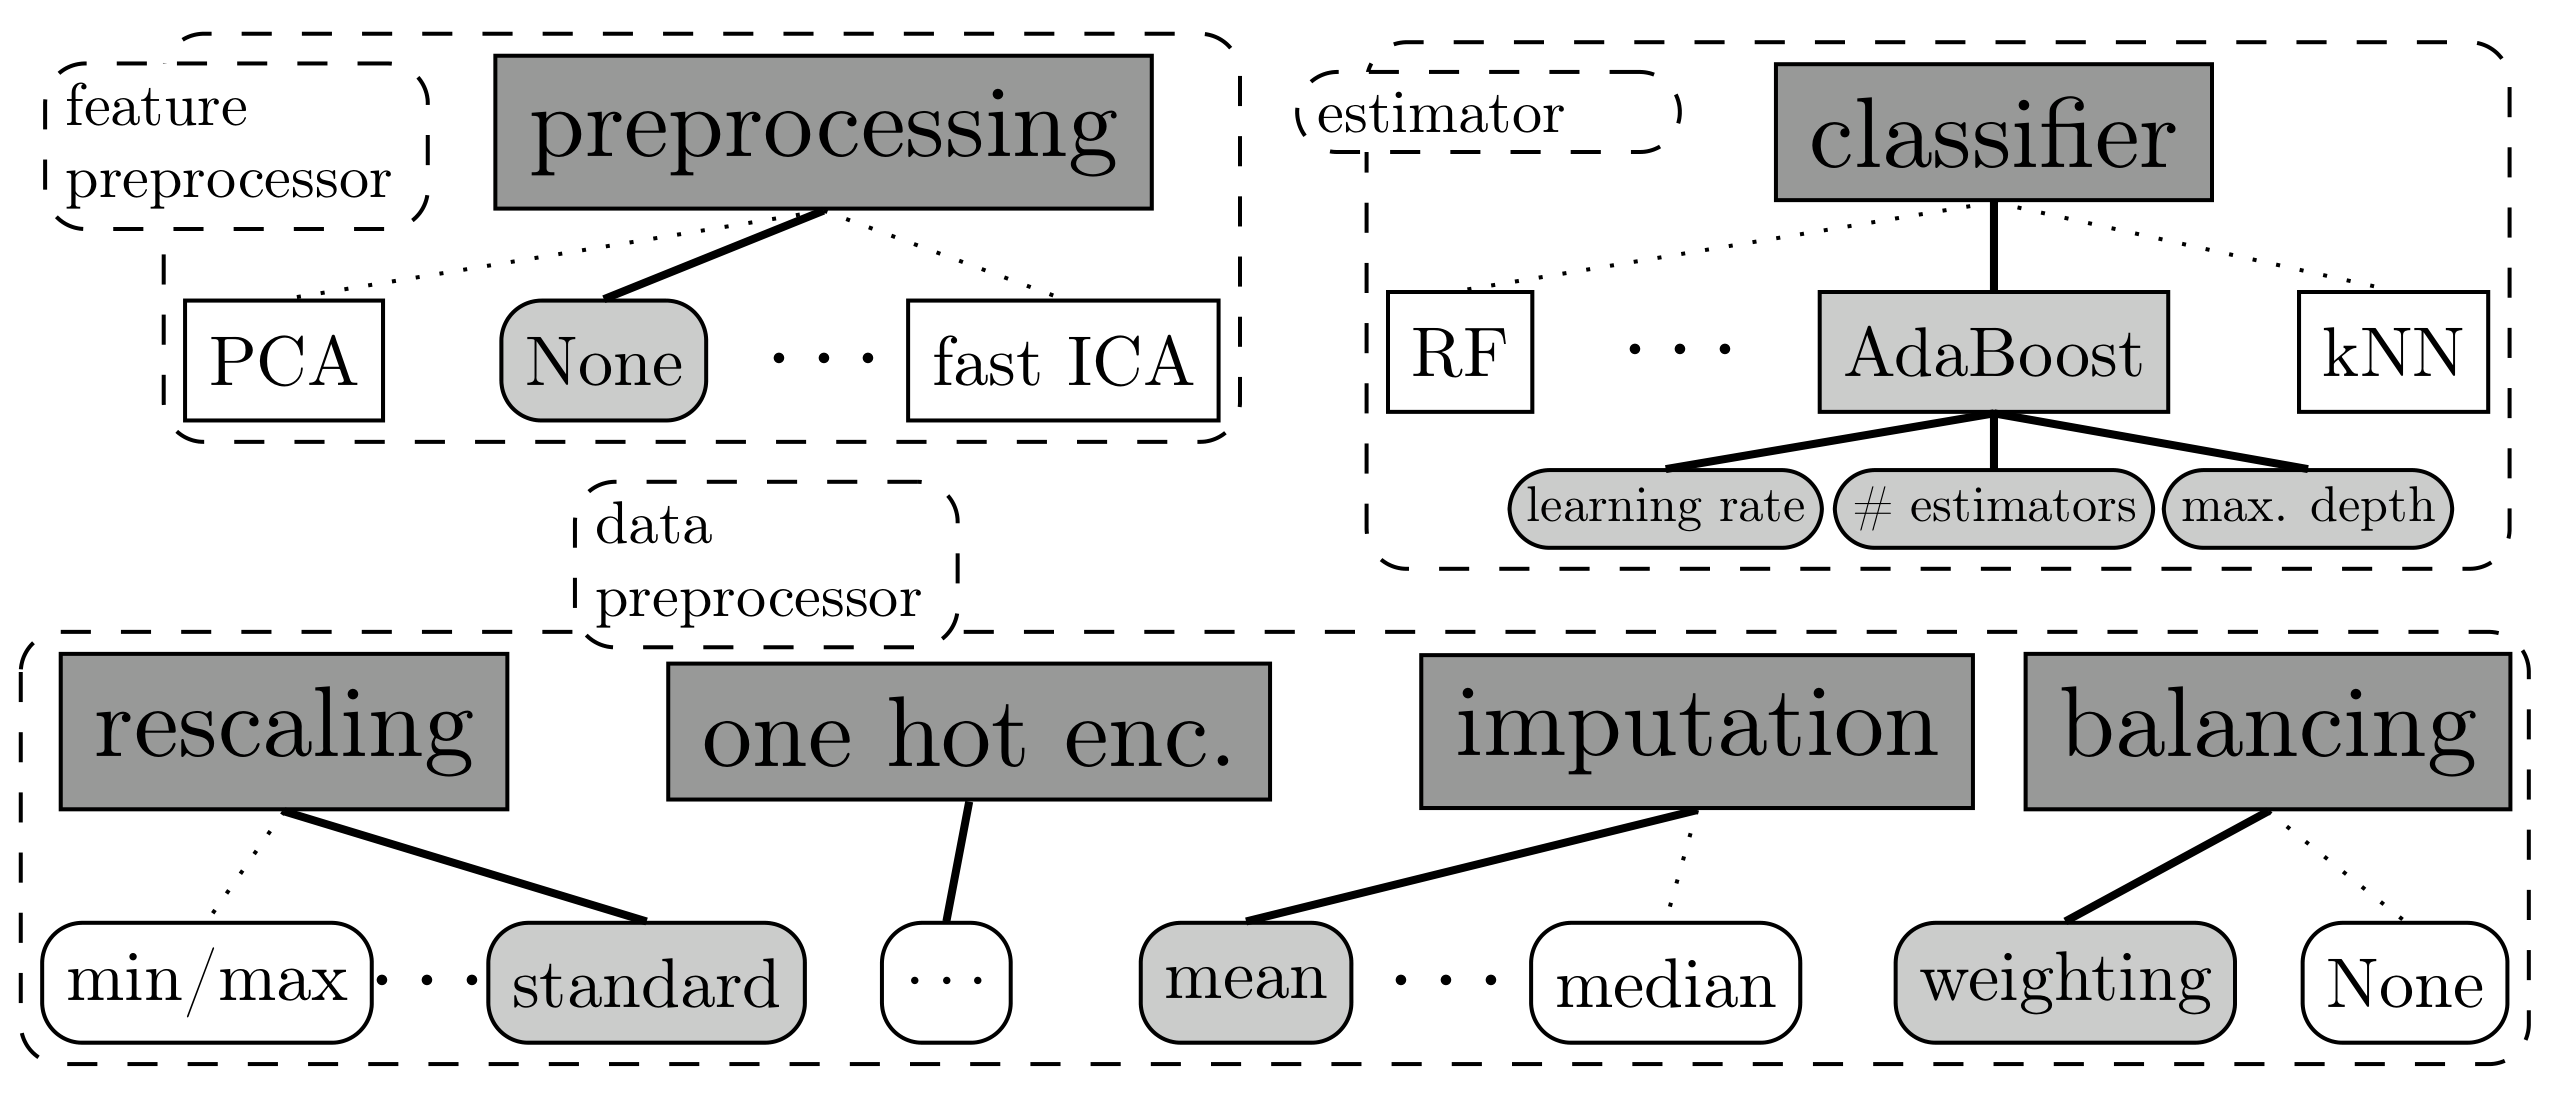
\includegraphics[width=.45\textwidth]{images/auto-sklearn}\footnote{\liturl{Feurer et al. 2015}{https://papers.nips.cc/paper_files/paper/2015/hash/11d0e6287202fced83f79975ec59a3a6-Abstract.html}}
    \end{center}
\end{frame}

%----------------------------------------------------------------------

\begin{frame}{Summary} 
\begin{enumerate}
    \item Hyperparameters occur in many different forms
    \item Hierarchical dependencies allow to encode the hyperparameter spaces of complex systems
    \item Determining what hyperparameters and values should be considered for optimization can be challenging in practice
\end{enumerate}
\end{frame}

\end{document}
